
\section{Rhythmic Similarity}\label{rhythmsimc}

This chapter provides an overview over some of the possibilities for computing music similarity by focusing on rhythmic features of different songs. \\
Nearly every MIR Toolkit provides an extraction tool for the beats per minute (BPM) and thus the tempo of each song. The most trivial solution to computing very low level rhythmic similarities is by sorting and comparing songs by their tempo. Of course there are far better and more accurate solutions. By just comparing the tempo of songs a lot of rhythm information is lost e.g. the rhythmic structures of songs like the time signature, up- and downbeats, etc.\\ 
This chapter presents some of the most promising approaches to compute rhythm similarities regarding the applicability in a big data framework.\\

\subsection{Beat histogram}\label{beathist}

Other similarity measurements are e.g. the usage of beat histograms as proposed by Tsanetakis and Cook \cite{rhythm3}. These are relatively similar to the later evaluated Rhythm Histograms.
Gruhne (et al.) further improved the beat histograms and suggested an additional post processing step for the beat histogram before calculating the similarity between songs with the euclidean distance, to improve a comparison of two songs with different tempi by transforming the beat histograms into the logarithmic lag domain. They found, that logarithmic re-sampling of the lag axis of the histogram and cross-correlation with an artificial rhythmic grid improves the performance of this similarity measurement further \cite[182]{rbh1}.
The essentia toolkit offers methods to extract the beat histogram. The different detected potential bpms are normalized to 1. If a song changes its tempo then multiple peaks can be seen.\\ 
Figure \ref{fig:bh1} shows the beat histograms of the song "Rock you like a hurricane" by the Scorpions and covered by Knightsbridge as well as two different versions of the song "Behind Space" from the swedish metal band In Flames, one is sung by Stanne Mikkels in 1994 and the second version was recorded with Anders Friden as a singer in 1999. The 1994 version changes its tempo in the outro of the song as can be seen in the figure.

\begin{figure}[htbp]
	\centering
	\framebox{\parbox{1\textwidth}{
			\begin{subfigure}{.495\textwidth}
				\centering
				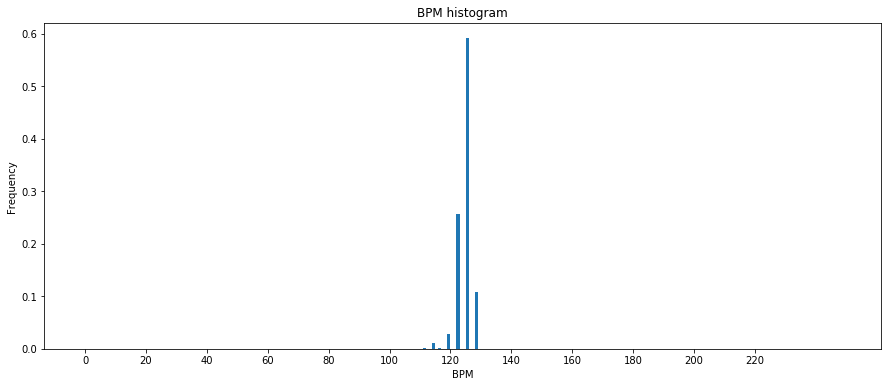
\includegraphics[scale=0.25]{Images/Beat/h_o_bh.png}
				\caption{Scorpions}
				\label{hobh}
			\end{subfigure}%
			\begin{subfigure}{.495\textwidth}
				\centering
				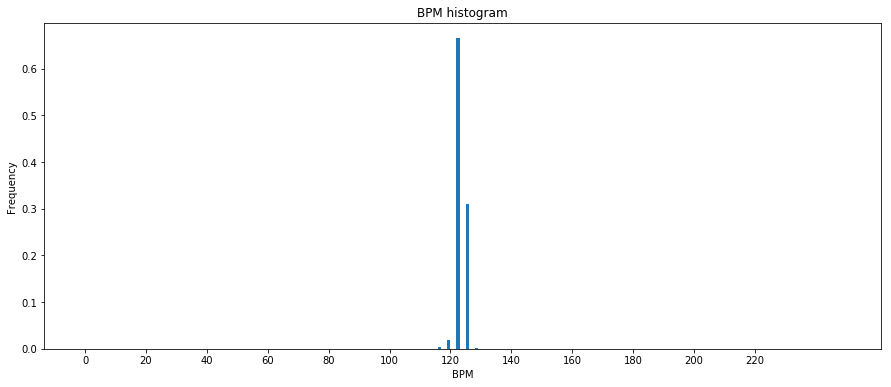
\includegraphics[scale=0.25]{Images/Beat/h_c_bh.png}
				\caption{Knightsbridge}
				\label{hcbh}
			\end{subfigure}% 
			
			\begin{subfigure}{.495\textwidth}
				\centering
				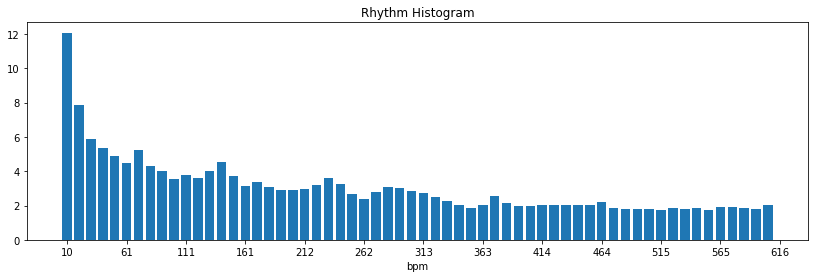
\includegraphics[scale=0.25]{Images/Beat/s_s_bh.png}
				\caption{94' Version Stanne}
				\label{ssbh}
			\end{subfigure}%
			\begin{subfigure}{.495\textwidth}
				\centering
				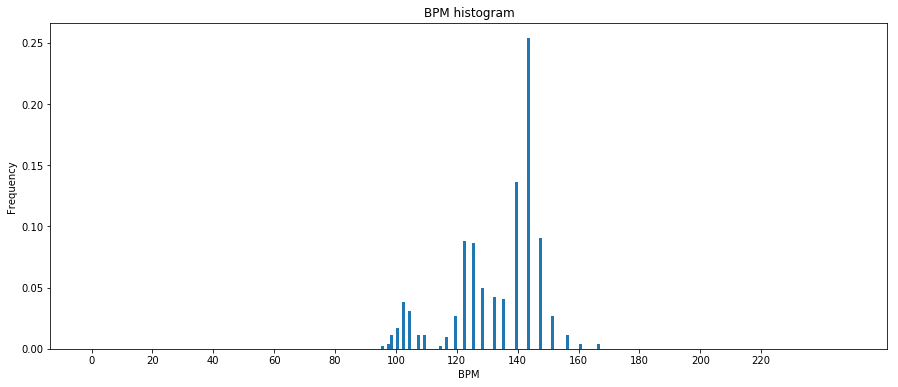
\includegraphics[scale=0.25]{Images/Beat/s_a_bh.png}
				\caption{99' Version Anders}
				\label{sabh}
			\end{subfigure}%			
	}}
	\caption{Beat Histogram}
	\label{fig:bh1}
\end{figure}

\FloatBarrier
 
Another feature that will just be mentioned here (one of the older ones from 2002) uses the beat spectrum as a feature \cite{rhythm1}.

\subsection{Rhythm patterns}

A more state-of-the-art feature is the so called rhythm pattern, also known as fluctuation patterns for instance mentioned by \cite{rp1}. 
To extract these features the rp\_extractor library \cite{rp_extract} was made publicly available by the TU Vienna \cite{rp_extract2}. Figure \ref{fig:rp1} shows the extracted rhythmic patterns of the previously mentioned songs "Rock you like a Hurricane" and "Behind Space". The similarities of the different versions from the same songs are quite visible while at the same time substantial differences between the different songs are recognizable.

\begin{figure}[htbp]
	\centering
	\framebox{\parbox{1\textwidth}{
			\begin{subfigure}{.495\textwidth}
				\centering
				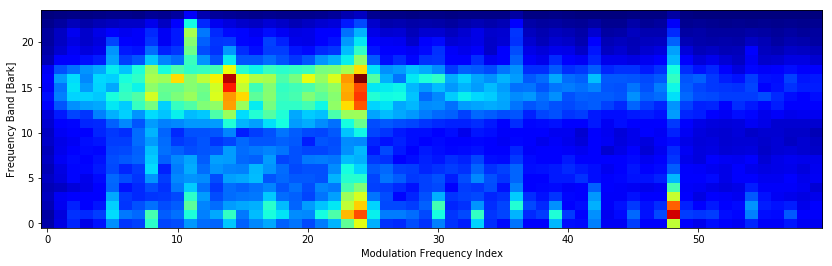
\includegraphics[scale=0.25]{Images/Beat/h_o_rp.png}
				\caption{Scorpions}
				\label{horp}
			\end{subfigure}%
			\begin{subfigure}{.495\textwidth}
				\centering
				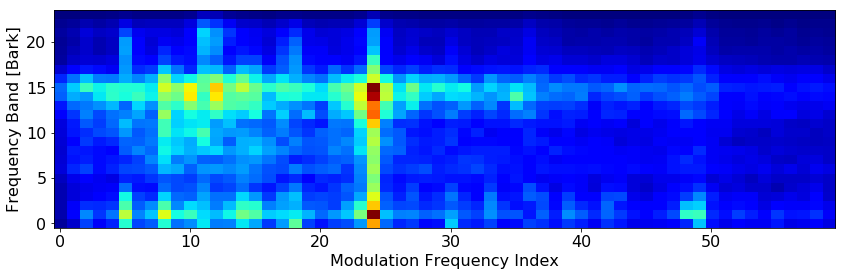
\includegraphics[scale=0.25]{Images/Beat/h_c_rp.png}
				\caption{Knightsbridge}
				\label{hcrp}
			\end{subfigure}% 
			
			\begin{subfigure}{.495\textwidth}
				\centering
				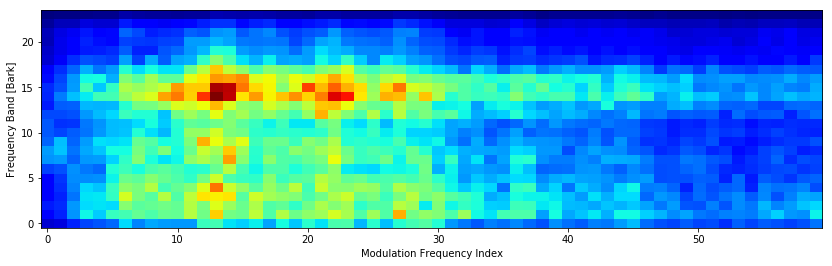
\includegraphics[scale=0.25]{Images/Beat/s_s_rp.png}
				\caption{94' Version Stanne}
				\label{ssrp}
			\end{subfigure}%
			\begin{subfigure}{.495\textwidth}
				\centering
				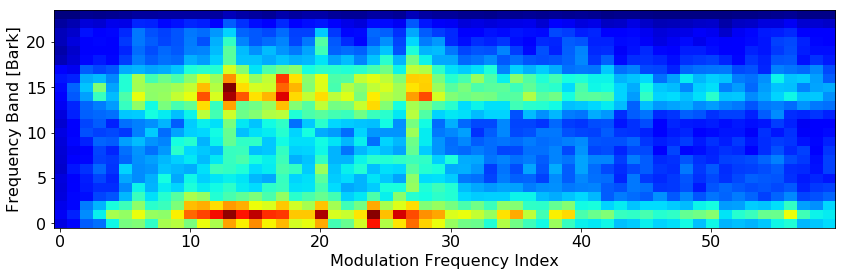
\includegraphics[scale=0.25]{Images/Beat/s_a_rp.png}
				\caption{99' Version Anders}
				\label{sarp}
			\end{subfigure}%			
	}}
	\caption{Rhythmic Patterns}
	\label{fig:rp1}
\end{figure}

\noindent The x-axis represents the frequency band converted to the bark scale (a scale representing the human auditory system comparable to the mel scale) and the y-axis represents the modulation frequency index representing the modulation frequencies up to 10Hz (600 BPM).
The Bark of a frequency $f$ can be determined using formula \ref{eq:bark}.
\begin{equation} \label{eq:bark}
Bark = 13 \arctan(0.00076 f) + 3.5 \arctan ((f / 7500)^2)
\end{equation}
The algorithm to extract the rhythm patterns as well as the rhythm histogram and statistical spectrum descriptors measuring the variations over the critical frequency bands can be seen in figure \ref{fig:rpe}.

\begin{center}
  % setting the typeface to sans serif and the font size to small
  % the scope local to the environment
  \sffamily
  \footnotesize
  \begin{tikzpicture}[auto,
    %decision/.style={diamond, draw=black, thick, fill=white,
    %text width=8em, text badly centered,
    %inner sep=1pt, font=\sffamily\small},
    block_center/.style ={rectangle, draw=black, thick, fill=white,
      text width=16em, text centered,
      minimum height=2em},
    block_left/.style ={rectangle, draw=black, thick, fill=white,
      text width=16em, text ragged, minimum height=2em, inner sep=6pt},
    block_noborder/.style ={rectangle, draw=none, thick, fill=none,
      text width=18em, text centered, minimum height=1em},
    block_assign/.style ={rectangle, draw=black, thick, fill=white,
      text width=18em, text ragged, minimum height=2em, inner sep=6pt},
    block_lost/.style ={rectangle, draw=black, thick, fill=white,
      text width=16em, text ragged, minimum height=2em, inner sep=6pt},
      line/.style ={draw, thick, -latex', shorten >=0pt}]
    % outlining the flowchart using the PGF/TikZ matrix funtion
    \matrix [column sep=5mm,row sep=3mm] {
      % enrollment - row 1
      \node [block_center] (audiosig) {Audio Signal};\\
      % enrollment - row 2
      \node [block_center] (pre) {Pre-Processing};\\
      % enrollment - row 3
      \node [block_center] (stft) {Power Spectrum (STFT)};\\ 
      % follow-up - row 4
      \node [block_center] (bark) {Critical Bands (Bark scale)};\\
      % follow-up - row 5
      \node [block_center] (phon) {Equal Loudness (Phon)};\\
      % follow-up - row 6
      \node [block_center] (sone) {Specific Loudness Sens. (Sone)};
	  & \node [block_assign] (stat) {Statistical Spectrum Descriptor $\rightarrow$ \textit{\textbf{SSD}}};\\
      % follow-up - row 7
	  \node [block_center] (fft) {Modulation Amplitude (FFT)};
 	  & \node [block_assign] (rh) {Rhythm Histogram $\rightarrow$ \textit{\textbf{RH}}};\\
       % follow-up - row 8
      \node [block_center] (fsw) {Fluctuation Strength Weighting};\\
      % follow-up - row 9
      \node [block_center] (filt) {Filtering/ Blurring};
   	  & \node [block_assign] (rp) {Rhythmic Patterns $\rightarrow$ \textit{\textbf{RP}}};\\
    };% end matrix
    % connecting nodes with paths
    \begin{scope}[every path/.style=line]
      % paths for enrollemnt rows
      \path (audiosig)   -- (pre);
      \path (pre)  -- (stft);
      \path (stft) -- (bark);
      \path (bark) -- (phon);
      \path (phon) -- (sone);
      \path (sone) -- (stat);
      \path (sone) -- (fft);
      \path (fft) -- (rh);
      \path (fft) -- (fsw);
      \path (fsw) -- (filt);
      \path (filt) -- (rp);
    \end{scope}
  \end{tikzpicture}
  	\captionof{figure}{Rhythm Pattern extraction \cite{rp_extract2}}
	\label{fig:rpe}
\end{center}

\noindent So in conclusion the Rhythm Patterns basically represent the BPM of various frequency bands.
To compare two different songs the euclidean distance between the vectorized rhythm pattern matrices can be calculated as Pampalk suggests \cite[p. 40]{fp1}\\
Pohle, Schnitzer et al. refined Fluctuation Patterns into Onset Patterns e.g. by using semitone bands instead of fewer critical bands to detect onsets. \cite{rp2}\\
This thesis however focuses on Fluctuation/ Rhythm patterns extracted with the rp\_extractor library. 

\subsection{Rhythm Histogram}

A more simplistic and lower dimensional feature coming with the rp\_extract toolkit is the Rhythm histogram. "The Rhythm Histogram features we use are a descriptor for general rhythmics in an audio document. Contrary to the Rhythm Patterns and the Statistical Spectrum Descriptor, information is not stored per critical band. Rather, the magnitudes of each modulation frequency bin of all 24 critical bands are summed up, to form a histogram of "rhythmic energy" per modulation frequency. The histogram contains 60 bins which reflect modulation frequency between 0 and 10 Hz." \cite[p. 3]{rp1}. 
The difference in comparison to the beat histogram mentioned earlier in section \ref{beathist} appears to be, that the beat histogram focuses on the basic tempo of the whole song while the rhythm histogram takes all frequency bands and therefor the sub-rhythms of single instruments into account. 

\begin{figure}[htbp]
	\centering
	\framebox{\parbox{1\textwidth}{
			\begin{subfigure}{.495\textwidth}
				\centering
				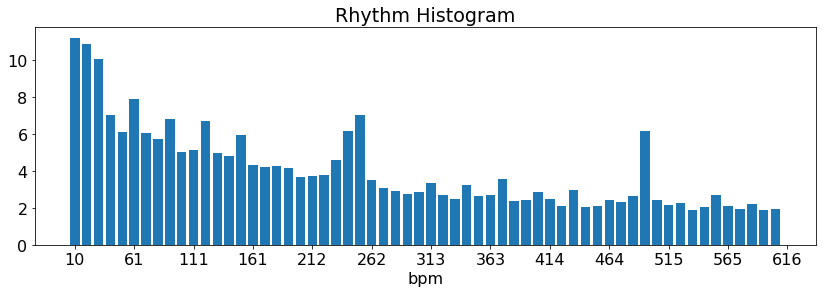
\includegraphics[scale=0.25]{Images/Beat/h_o_rh.png}
				\caption{Scorpions}
				\label{horh}
			\end{subfigure}%
			\begin{subfigure}{.495\textwidth}
				\centering
				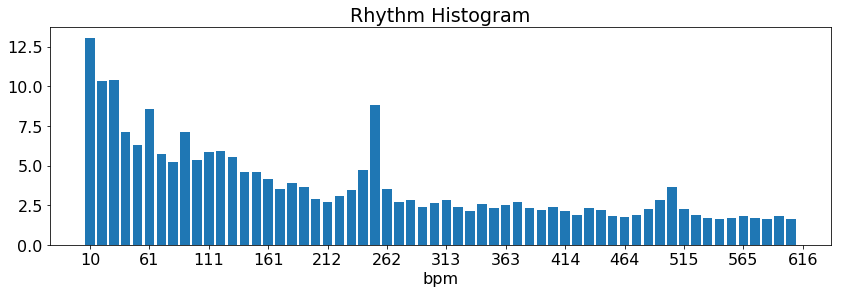
\includegraphics[scale=0.25]{Images/Beat/h_c_rh.png}
				\caption{Knightsbridge}
				\label{hcrh}
			\end{subfigure}% 
			
			\begin{subfigure}{.495\textwidth}
				\centering
				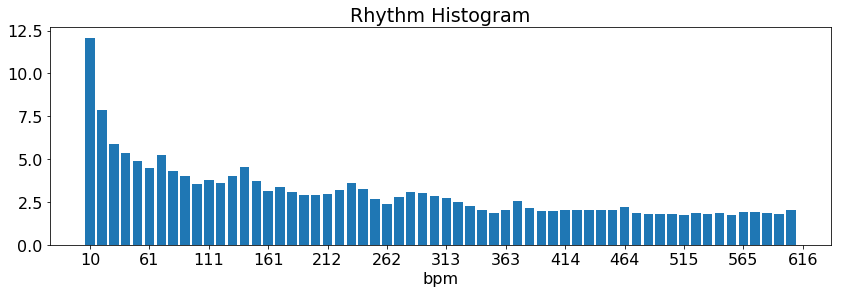
\includegraphics[scale=0.25]{Images/Beat/s_s_rh.png}
				\caption{94' Version Stanne}
				\label{ssrh}
			\end{subfigure}%
			\begin{subfigure}{.495\textwidth}
				\centering
				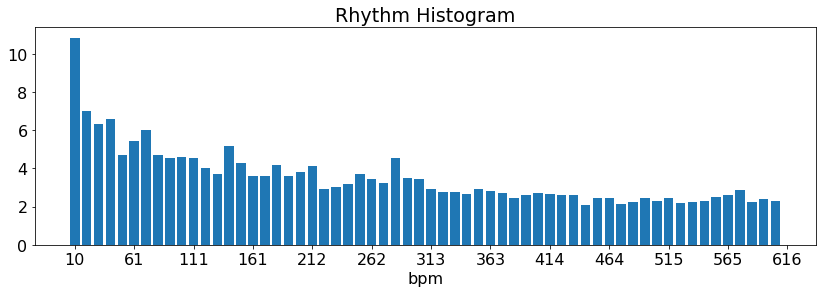
\includegraphics[scale=0.25]{Images/Beat/s_a_rh.png}
				\caption{99' Version Stanne}
				\label{sarh}
			\end{subfigure}%			
	}}
	\caption{Rhythm Histogram}
	\label{fig:rh1}
\end{figure}

\subsection{cross-correlation}

Estimating the onset strength per beat and creating a discrete-time signal for each song is an other option. Similar to the chroma features the cross-correlation of the onset functions could be used as a similarity measurement. 

\begin{figure}[htbp]
	\centering
	\framebox{\parbox{1\textwidth}{ 			
			\begin{subfigure}{.495\textwidth}
				\centering    
				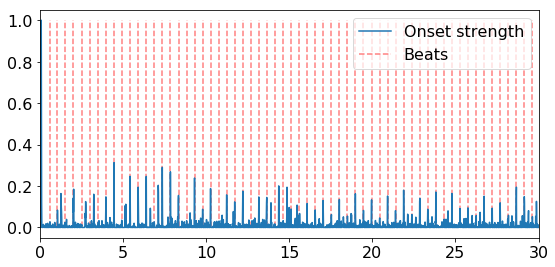
\includegraphics[scale=0.3]{Images/Beat/h_o_on.png}
				\caption{Scorpions}
				\label{hoon}
			\end{subfigure}		
			\begin{subfigure}{.495\textwidth}
				\centering     
				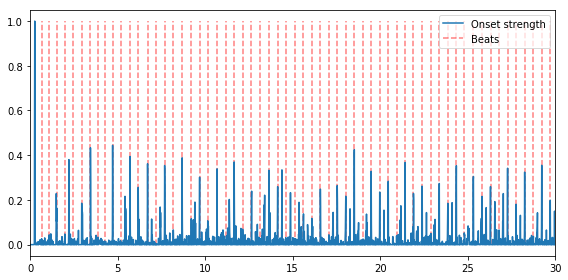
\includegraphics[scale=0.3]{Images/Beat/h_c_on.png}
				\caption{Knightsbridge}
				\label{hcon}
			\end{subfigure}%	
				
			\begin{subfigure}{.495\textwidth}
				\centering    
				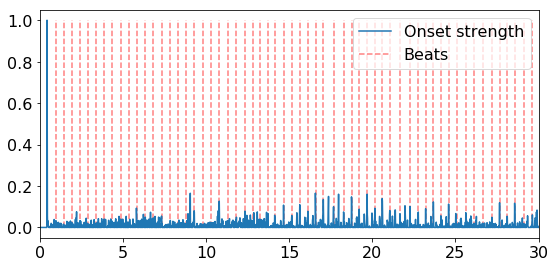
\includegraphics[scale=0.3]{Images/Beat/s_s_on.png}
				\caption{94' Version Stanne}
				\label{saon}
			\end{subfigure}		
			\begin{subfigure}{.495\textwidth}
				\centering     
				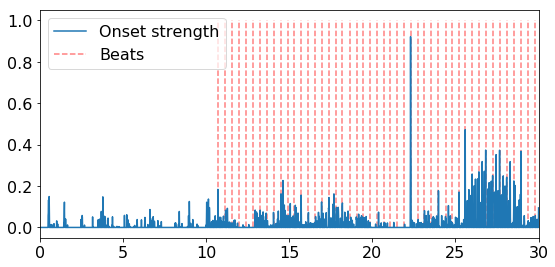
\includegraphics[scale=0.3]{Images/Beat/s_a_on.png}
				\caption{99' Version Stanne}
				\label{sson}
			\end{subfigure}%			
				
	}}
	\caption{Detected Onsets (first 30 seconds)}
	\label{fig:ons1}
\end{figure}	

\noindent Looking at the extracted onset features of the Song "Behing Space" by In Flames (sung by Anders Frieden 99' and Stanne Mikkels 94') in figure \ref{fig:ons1}, one can see that the quality of these signals are greatly dependent on the underlying beat extraction and onset detection algorithms. E.g. the librosa toolkit struggles to detect beats in the first 10 seconds of the version of the song from the year 1999. Also this representation seems to contain a lot less valuable and comparable information in contrast to Fluctuation Patterns. 
In conclusion this approach is discarded and not further considered and tested in this thesis.  

\section{Summary}\label{sumfeat}

\subsection{Timbre Similarity}

Three different similarity metrics are chosen: 
\begin{itemize}
	\setlength\itemsep{-0.5em}
	\item Euclidean Distance
	\item Symmetric Kullback-Leibler Divergence
	\item Jensen-Shannon like Divergence
\end{itemize}
To calculate the distances, for each song the mean vector, variance and covariance matrix has to be computed for each mfcc band. These are stored in two different output text files: 
\begin{itemize}
	\setlength\itemsep{-0.5em}
	\item out.mfcc (containing mean vector (length $b$), variance vector (length $b$) and vectorized upper triangular covariance matrix (length $b$))
	\item out.mfcckl (containing mean vector (length $b$) and full covariance matrix as a vector (length $\frac{b \cdot (b-1)}{2}$))
\end{itemize}
The amount of chosen mfcc bands is $b = 13$.\\
The second file is created to get rid of the necessity to rearrange the covariance matrix inside the Big Data Framework and reduce the computation time when a similarity computation request is processed.
The text files contain strings like the following:\\
\textit{music/CHANDELIER2.mp3; [-498.03763,  ... ,4.321189]; [8943.487,... ,61.624344]; [ 8944.3907652, ... ,74.17548092]}\\
\textit{music/CHANDELIER2.mp3; [-498.03763,  ... ,4.321189]; [8943.487,... ,61.624344]; [[6568.27958735, ... ,74.64776425], ... , [74.64776425, ... ,69.1589048]]}

\subsection{Melodic Similarity}

Two different similarity metrics are chosen: 
\begin{itemize}
	\setlength\itemsep{-0.5em}
	\item Levenshtein Distance
	\item cross-correlation on full beat aligned and per beat averaged chroma features, key shifted to A
\end{itemize}
These are stored in two different output text files. The vector length is dependent on the numbers of detected beats $n$
\begin{itemize}
	\setlength\itemsep{-0.5em}
	\item out.notes (containing the estimated original key, the scale and a list of most dominant key per beat, key shifted to the A key (length $n$))
	\item out.chroma (full beat aligned chromagram, containing a $12 \times n$ matrix)
\end{itemize}
The output files contain strings like follows:\\
\textit{music/CHANDELIER2.mp3; G; minor; [6, 2, 5, 7, 7, 7, 7, 2, 2, 2, 2, 2, 0, 0, 0, 0, 3, 0, 0, 0]}\\
\textit{music/CHANDELIER2.mp3; [[0.5209161 ,0.82440507,... ,0.68443549] ... [0.31470749,0.02552716,... ,0.01234249]]}
for the out.notes files and out.chroma files. 

\subsection{Rhythm Similarity}

Three different similarity metrics are chosen: 
\begin{itemize}
	\setlength\itemsep{-0.5em}
	\item euclidean distance between beat histograms
	\item euclidean distance between rhythm histograms
	\item euclidean distance between rhythm patterns
\end{itemize}
These are stored in three different output text files.
\begin{itemize}
	\setlength\itemsep{-0.5em}
	\item out.bh (containing the estimated overall bpm and a vector for the beat histogram normalized to one (length $250$))
	\item out.rh (containing a vector for the rhythm histogram extracted with rp\_extract (length $60$))
	\item out.rp (containing a vectorized matrix for the rhythm patterns extracted with rp\_extract (length $24 \times 60$))
\end{itemize}
The text files contain strings like:\\
\textit{music/CHANDELIER2.mp3; 86.9380264282; [0. ... 0.01453488 ...  0.  0.]}\\
\textit{music/CHANDELIER2.mp3,15.2521291416,10.10441871, ... ,2.2519330706}\\
\textit{music/CHANDELIER2.mp3,0.0237481782333,0.0208784207788, ... ,0.00204177442894}\\